\documentclass[12pt]{article}
% Эта строка — комментарий, она не будет показана в выходном файле
\usepackage{ucs}
\usepackage[warn]{mathtext}
\usepackage[utf8x]{inputenc} % Включаем поддержку UTF8
\usepackage[russian]{babel}  % Включаем пакет для поддержки русского языка
\usepackage{amsmath}
\usepackage{mathtools}
\usepackage{amssymb}
% \usepackage[dvips]{graphicx}
% \graphicspath{{noiseimages/}}
\usepackage[pdftex]{graphicx}


% Параметры страницы: 1см от правого края и 2см от остальных.


\hoffset=0mm
\voffset=0mm
\textwidth=180mm        % ширина текста
\oddsidemargin=-6.5mm   % левое поле 25.4 - 5.4 = 20 мм
\textheight=240mm       % высота текста 297 (A4) - 40
\topmargin=-15.4mm      % верхнее поле (10мм)
\headheight=5mm      % место для колонтитула
\headsep=5mm          % отступ после колонтитула
\footskip=8mm         % отступ до нижнего колонтитула


\begin{document}
    \author {Жарков Андрей 495}
    \title {Лабораторная работа 2.6 \\  Определение энергии активации по температурной зависимости вязкости жидкости.}
    \maketitle{}
    
    \begin{center}
    	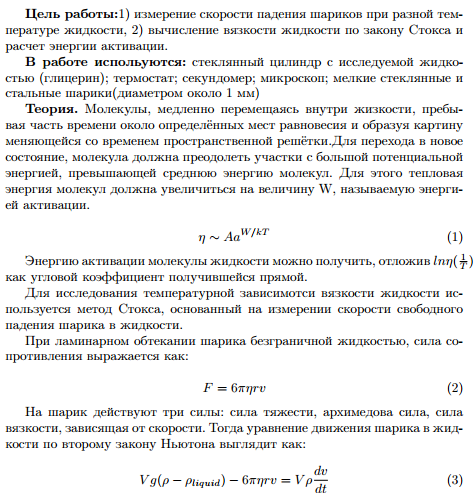
\includegraphics[width=14cm]{theory1.png}
    	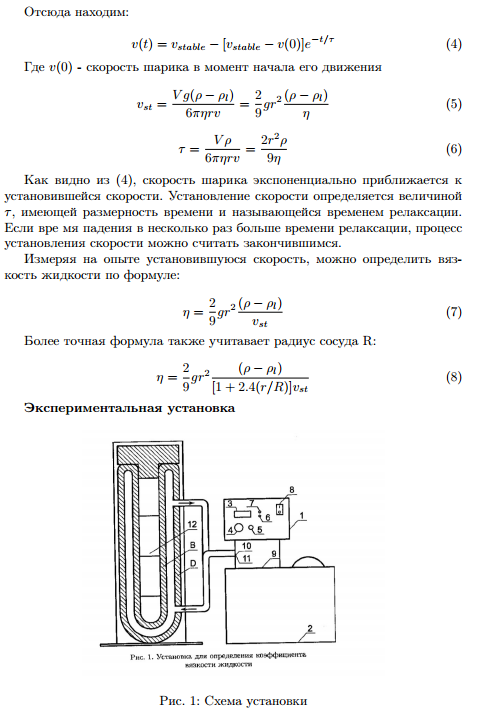
\includegraphics[width=14cm]{theory2.png}
    	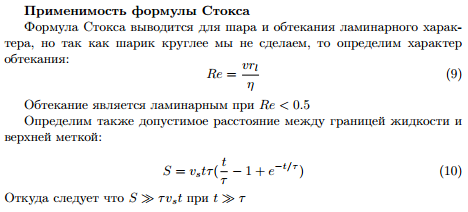
\includegraphics[width=14cm]{theory3.png}
    \end{center}
    
    %\textbf{Цель работы:} 1) измерение скорости падения шариков при разной температуре жидкости; 2) вычисление вязкости жидкости по закону Стокса и расчёт энергии активации.
    
    
    %\textbf{В работе используются:} стеклянный цилиндр с исследуемой жидкостью (глицерин); термостат; секундомер; горизонтальный компаратор; микроскоп; мелкие шарики (диаметром около 1мм).
    
    %\begin{center}
    	%\textbf{\large{Теоретическое введение.}}
    	%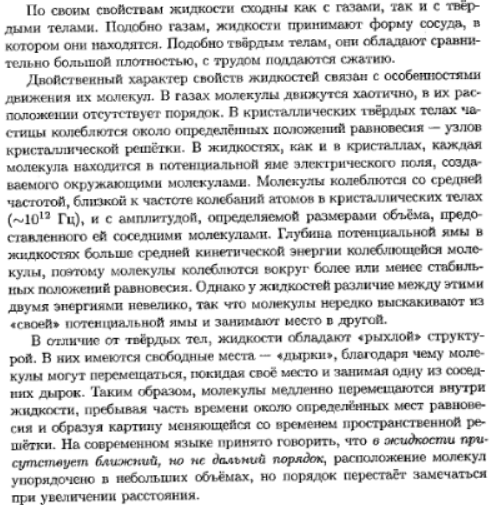
\includegraphics[width=14cm, height=13cm]{theory_0.png}
    	%%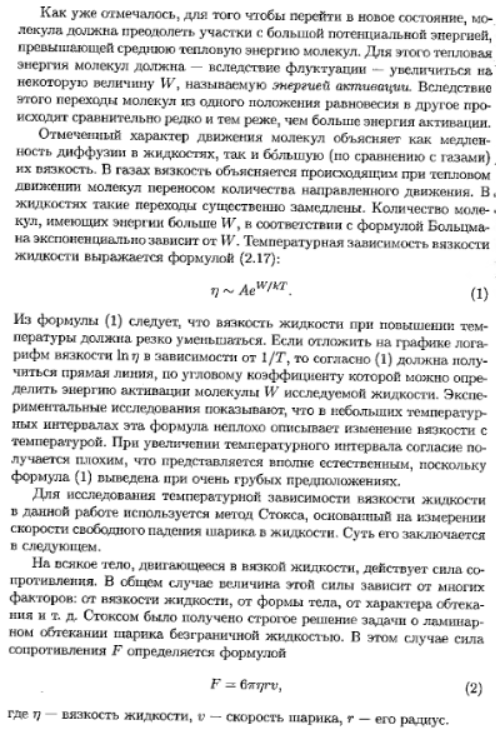
\includegraphics[width=16cm]{theory_1.png}
    	%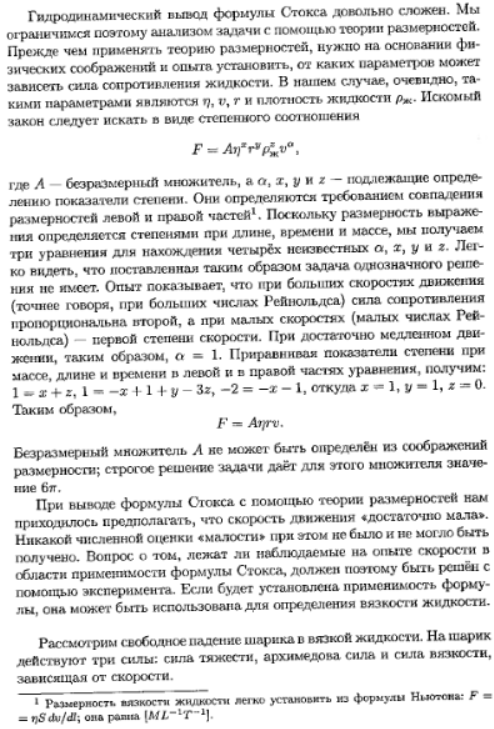
\includegraphics[width=16cm]{theory_2.png}
    	%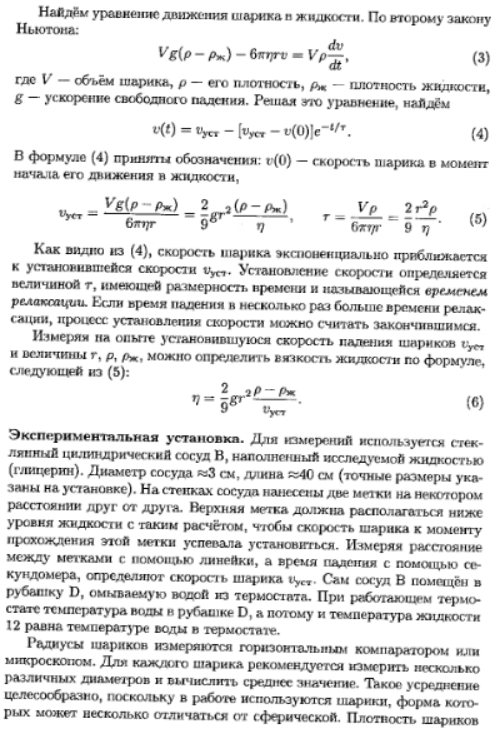
\includegraphics[width=16cm]{theory_3.png}
    	%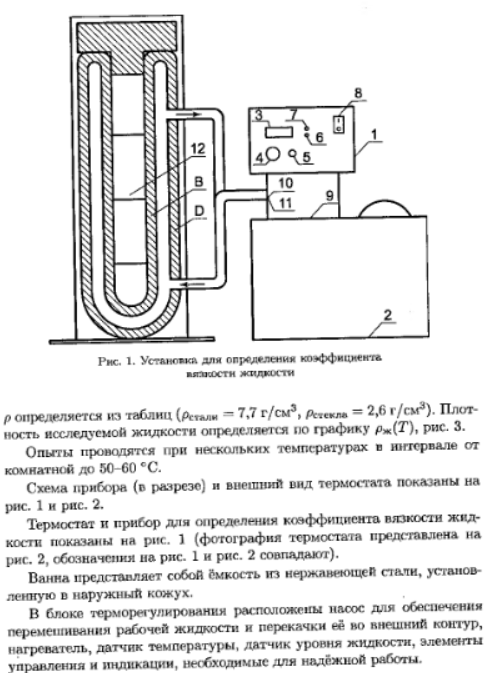
\includegraphics[width=16cm]{theory_4.png}
    	%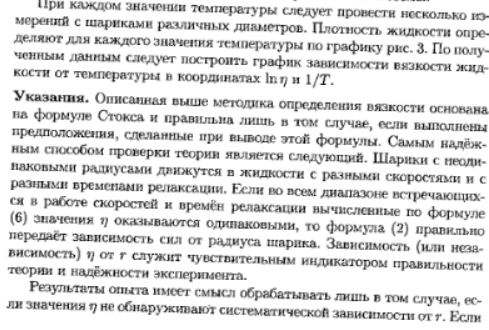
\includegraphics[width=16cm]{theory_5.png}
    	%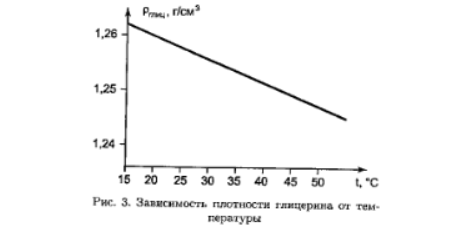
\includegraphics[width=16cm]{theory_6.png}
    	%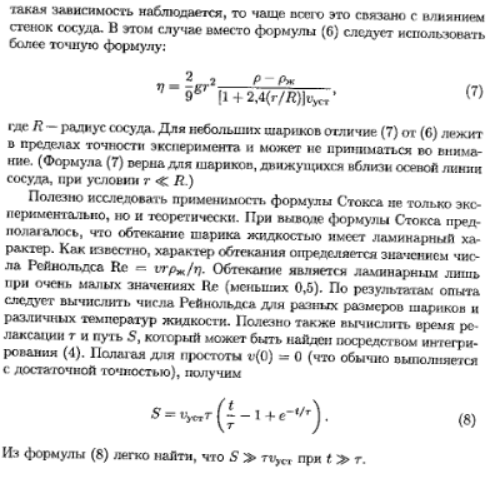
\includegraphics[width=16cm]{theory_7.png}
    	%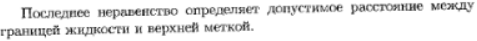
\includegraphics[width=16cm]{theory_8.png}
    %\end{center}
    
    \begin{center}
    	\textbf{\large{Выполнение работы}}
    \end{center}
    
    Будем бросать в жидкость шарики c известной плотностью у которых мы померили радиус. Измерив время прохождения участка длинны $L=9,8cm$ посчитаем установившуюся скорость шариков. Используя это, вычислим вязкость по формуле (7) - $\eta$ и (8) - $\eta_2$ и число рейнольдса $Re = \frac{\rho_{ж} v_{уст} r}{\eta}$, а также время релаксации $\tau$ (по формуле (6)) и путь релаксации $S=v_{уст}\tau$ для каждого из шариков.
    
    Погрешности при измерении: $\sigma_T = 0,1K$, $\sigma_r = 0,02mm$, $\sigma_t = 0,3c$
    
    \begin{center}
    	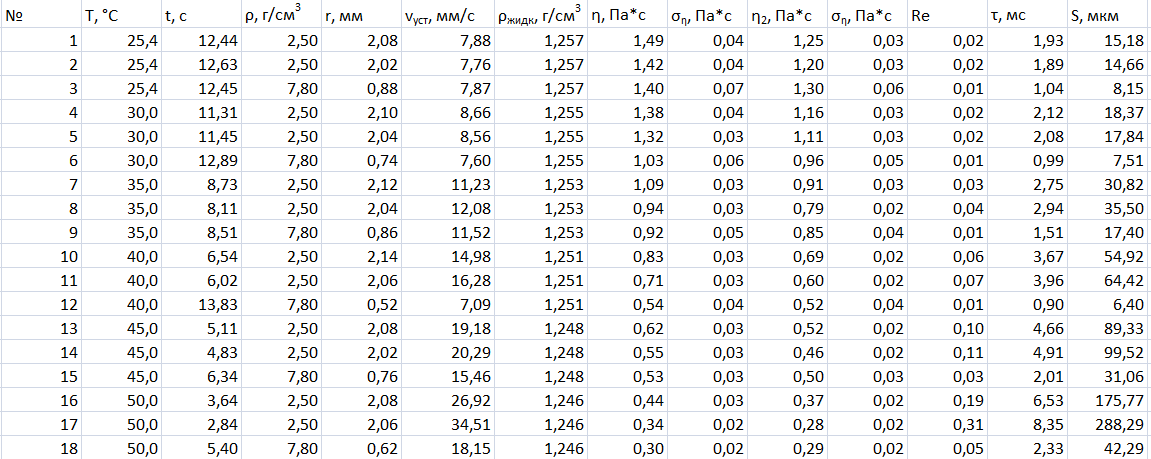
\includegraphics[width=18cm]{table1.png}
    \end{center}
    
    Как видим $\eta$ вообще говоря, зависит от $\rho$, поэтому в расчётах будем использовать $\eta_2$, вычисленное по формуле (8).
    
    Построим график $ln\eta(\frac{1}{T})$
    
    \begin{center}
    	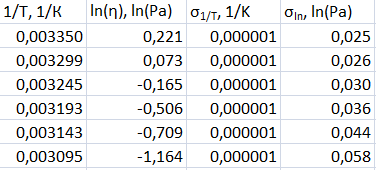
\includegraphics[width=7cm]{table2.png}\\
    	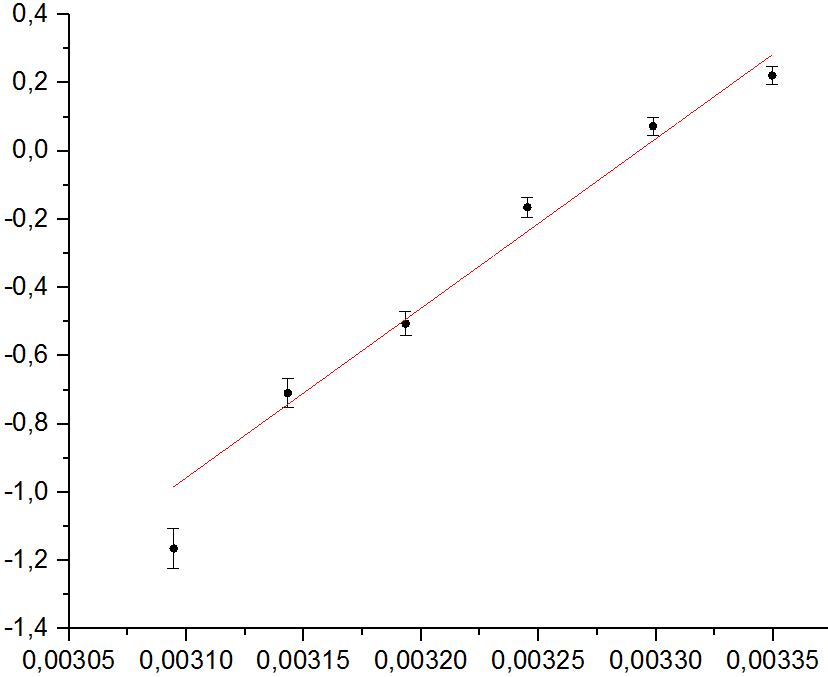
\includegraphics[width=14cm]{graph1.png}
    \end{center}
    
    Разброс точек достаточно заметный, это может быть связано с на самом деле далеко не шараобразной формой шариков.
    
    Найденный коэффициент наклона $\alpha = (50 \pm 4) * 100$, тогда
    
    Энергия активации $W = \alpha k = (6,9 \pm 0,5) * 10^{-20} Дж$
\end{document}